% \section{Introduction}


Vision-Language-Action (VLA) models have emerged as a powerful paradigm for general-purpose robotic manipulation with large-scale internet-level pretraining. By directly mapping observations to control signals, they provide a powerful foundation for executing complex motor skills. 
% However, despite their reactive proficiency, current VLA models are fundamentally limited by their Markovian nature. As the policy typically operates on a short temporal window of observations $p(a_t | o_t, l)$, it lacks the necessary capacity to maintain long-term consistency or benefit from past experiences, causing them to struggle in long-horizon tasks where past context dictates current actions.
% Vision-Language-Action (VLA) models have established a new baseline for robotic manipulation by providing a versatile foundation for executing diverse motor skills. By distilling multimodal data into a direct observation-to-action mapping, they enable robots to interact with the physical world with unprecedented dexterity.
Most existing architectures rely on the Markov assumption, where the policy $p(a_t | o_t, l)$ is conditioned only on the transient observation at the current time step. This inherent limitation prevents them from maintaining a persistent belief of the environment in non-Markovian settings. 
Consequently, VLAs struggle with complex, long-horizon tasks that demand long-range temporal dependencies, where the optimal action depends on a chain of past events or latent information that is no longer visible in the current sensory stream.
% Consequently, VLAs struggle with complex, long-horizon tasks, which requiring such as tracking hidden object states, adapting to dynamic environmental perturbations, or reconciling evolving human preferences within a multi-step execution chain.
% However, despite their reactive proficiency, current VLAs primarily function as memoryless executors. They typically operate on transient observations $p(a_t | o_t, l)$, which prevents them from maintaining a persistent belief of the environment in non-Markovian settings. Consequently, VLAs struggle with tasks requiring long-term logical consistency, such as managing hidden object states, adapting to dynamic environmental changes, or integrating evolving human preferences into a multi-step execution chain.


% To break the temporal constraints of reactive policies, recent research has explored expanding the observation context through auxiliary losses \cite{torne2025} or finetuning foundation models with native memory capabilities \cite{fang2025}. While these methods extend the history length, they predominantly adopt a \textbf{flat architecture} that forces the action predictor to resolve low-level sensory details and high-level strategic reasoning within the same computational manifold. This leads to an inherent \textbf{granularity conflict}: reactive control demands high-frequency, raw sensory precision to ensure physical stability, whereas strategic planning requires low-frequency, semantic abstraction to maintain logical coherence. Forcing a high-bandwidth VLA to process an ever-growing, noisy historical context not only incurs prohibitive computational overhead but also causes the policy to deviate under the distraction of irrelevant sensory cues.

% We argue that scaling robotic memory requires more than just longer contexts; it necessitates a \textbf{Hierarchical Memory Management} architecture that decouples execution from cognition. Inspired by the dual-process theory in cognitive science, we propose a tripartite system. At the base, a high-frequency \textbf{VLA} maintains reactive control stability. In the middle, an \textbf{Observer} acts as a cognitive gatekeeper, filtering transient sensory streams into discrete, task-relevant events. At the top, a \textbf{Planner} intervenes asynchronously to perform deep reasoning and memory retrieval. This decoupling allows the agent to protect high-level strategic consistency from low-level perceptual noise, ensuring that long-term knowledge is invoked only at critical junctions.


\begin{figure}
    \centering
    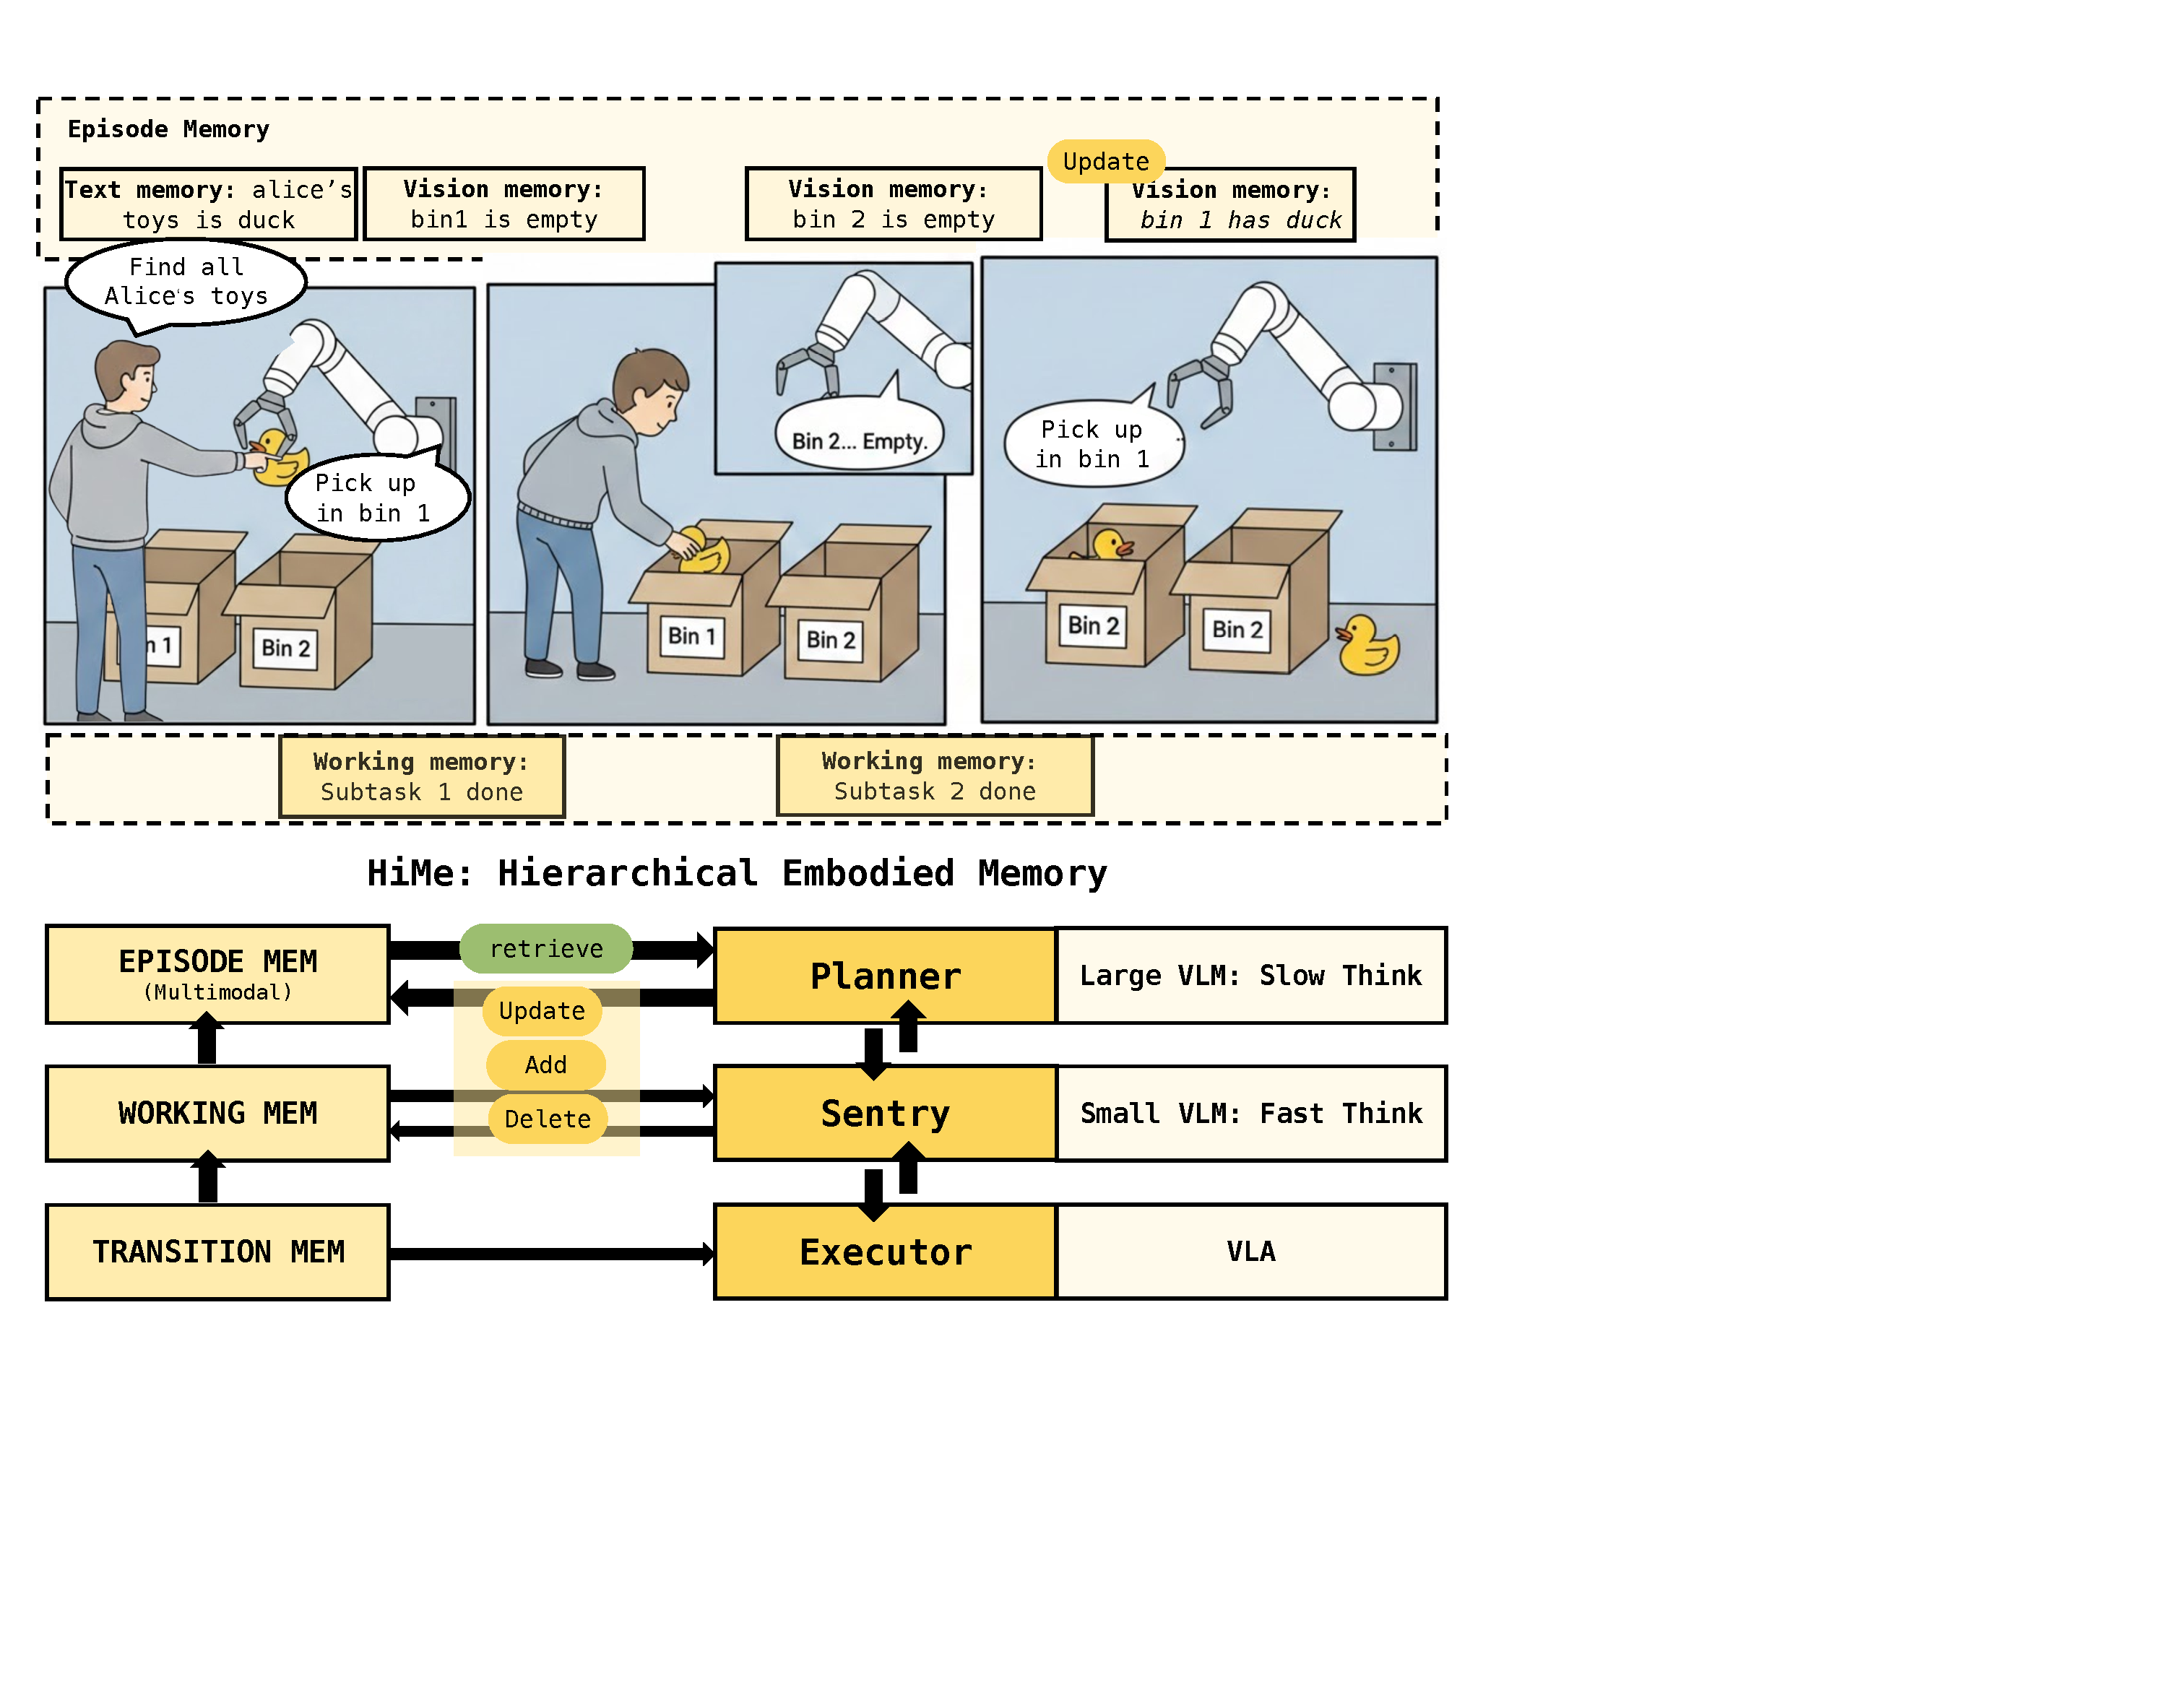
\includegraphics[width=1\linewidth]{imgs/intro.pdf}
    \caption{\textbf{Overview of HiMe.} A motivating example (top) illustrates the need for maintaining and updating task-relevant multimodal memory across long-horizon subtasks. HiMe addresses this challenge by organizing embodied intelligence into a hierarchical structure that separates fast execution from memory-driven reasoning over long time scales. }
    \label{fig:intro}
\end{figure}

% To break the temporal constraints of reactive policies, recent research has explored expanding the observation context. Some approaches utilize auxiliary losses \cite{torne2025} or finetuning to imbue models with native memory capabilities \cite{fang2025}. A notable advancement is MemER \cite{memer2025}, which retrieves historical trajectories and prepends them as visual context for a Vision-Language Model (VLM). However, these methods—including MemER—predominantly adopt a \textbf{flat memory paradigm}. They treat historical data as a static, unmanaged sequence, forcing the model to resolve low-level sensory details and high-level strategic reasoning within the same computational manifold. This leads to an inherent \textbf{granularity conflict}: reactive control demands high-frequency sensory precision, whereas strategic planning requires low-frequency semantic abstraction. Forcing a policy to process an ever-growing, uncurated historical context not only incurs prohibitive computational overhead but also causes the agent to deviate under the distraction of irrelevant sensory noise.

% To overcome these limitations, one intuitive approach is to imbue VLA models with native memory capabilities through specialized training or auxiliary losses \cite{torne2025, fang2025}. However, these training-based methods are often constrained by limited context windows and the inherent difficulty of optimizing long-range causal dependencies over hundreds of steps. Another alternative is to introduce Large Vision-Language Models (VLMs) as high-level memory containers to store and retrieve historical trajectories \cite{memer2025}. Yet, this strategy encounters a fundamental frequency-capability paradox: Utilizing massive, state-of-the-art VLMs for real-time planning introduces prohibitive computational latency that is misaligned with the high-frequency requirements of robotic control. Conversely, opting for smaller, distilled models to reduce latency often requires intensive domain-specific finetuning and inevitably strips the agent of the "slow-thinking" capability—the broad, cross-domain reasoning and zero-shot planning inherent in large-scale models. 

To overcome these limitations, one intuitive approach is to imbue VLA models with native memory capabilities through specialized training or auxiliary losses \cite{Torne2025LearningLD,Fang2025SAM2ActIV}. However, these training-based methods are often constrained by limited context windows and the inherent difficulty of optimizing long-range causal dependencies over hundreds of steps. Another alternative is to introduce Large Vision-Language Models (VLMs) as high-level memory containers to store and retrieve historical trajectories \cite{Sridhar2025MemERSU}. Yet, real-time robotic control imposes a strict upper bound on the deployable VLM scale, as control demands high-frequency, low-latency execution. This scale constraint, in turn, limits the internal world knowledge and generalization capabilities of the VLM, weakening its zero-shot performance. Importantly, most memory operations do not intrinsically require high-level reasoning or broad generalization. 

Motivated by this temporal and scale mismatch, we decouple memory and reasoning operations into hierarchical layers with distinct time scales.
% These observations suggest that the bottleneck of robotic memory is not merely a matter of model scale, but rather an architectural misalignment.
We propose \textbf{HiMe}, a \textbf{Hierarchical Embodied Memory} framework that decouples embodied intelligence into three functional layers with distinct temporal resolutions, mirroring the multi-store structure of human cognition. 
(1) The \textbf{Executor (VLA)} governs \textbf{transient memory}, focusing on high-frequency sensory-motor coordination for physical stability. 
(2) The \textbf{Sentry} acts as the guardian of \textbf{working memory} (short-term memory); it asynchronously filters the continuous sensory stream to identify critical state transitions, effectively bridging the gap between raw perception and semantic events. 
(3) The \textbf{Planner} manages \textbf{episodic memory} (long-term memory). 
By invoking the ``slow-thinking" Planner only at the discrete junctions identified by the Sentry, our architecture preserves deep strategic reasoning while maintaining real-time execution, effectively resolving the frequency-capability paradox.

% Inspired by the multi-store model of human cognition, we propose a \textbf{Hierarchical Memory Management} framework that decouples execution from cognition across three distinct temporal scales. At the base, the \textbf{Executor (VLA)} maintains high-frequency reactive control, modeling \textbf{transient memory} for immediate physical stability. Above this, a \textbf{Monitor} acts as the guardian of \textbf{working memory}; it asynchronously tracks task progress and filters the continuous sensory stream into discrete, task-relevant events. At the apex, a \textbf{Planner} manages \textbf{episodic memory} (long-term experience). The Planner is only invoked at critical junctions identified by the Monitor, allowing it to perform deep reasoning and memory retrieval without interfering with the high-speed execution loop. This hierarchical decoupling ensures that strategic consistency is preserved while maintaining real-time responsiveness.



% However, a static memory hierarchy is insufficient for the complexities of real-world human-robot interaction, which is characterized by \textbf{multimodal richness} and \textbf{high dynamism}. Human instructions often carry dense logical constraints and safety preferences---such as ``this tool is fragile, handle it with care''---which are nearly impossible to capture through vision-only trajectories alone. Furthermore, in open-ended environments, task goals and human preferences are not static; they evolve. A memory system that only supports passive accumulation, such as MemER \cite{memer2025}, inevitably suffers from knowledge stagnation and cognitive dissonance when faced with outdated or conflicting experiences.


However, a static memory hierarchy alone is insufficient for the complexities of real-world human-robot interaction, which is characterized by: (1) \textit{multimodal richness}, where human instructions carry dense logical constraints and latent preferences---such as designating a specific red cup as ``Alice's cup''---that are nearly impossible to capture through vision-only trajectories; and (2) \textit{high dynamism}, where task goals and environment states are not static but evolve. A memory system that only supports passive accumulation~\cite{Sridhar2025MemERSU} inevitably suffers from knowledge stagnation and cognitive dissonance when faced with such outdated or conflicting experiences.

Furthermore, our Hierarchical Memory framework treats memory as a multimodal, dynamic knowledge system centered around two fundamental dimensions:

\textit{(1) What to memorize?: Cross-modal Semantic Schemata.} To bridge the gap between raw perception and logical intent, we represent episodic memory as an object-centric system where visual experiences are deeply anchored with high-density textual descriptions. This organization allows the Planner to retrieve not only visual features but also the underlying ownerships, procedural rules, and human preferences that are invisible in pure pixel space.

\textit{(2) How to memorize?: Active Management Mechanism.} In contrast to passive storage, we introduce explicit \textit{Add}, \textit{Update}, and \textit{Delete} operations to grant the robot knowledge plasticity. When the Sentry detects a significant state transition or a revision in user intent, the Planner proactively refines the knowledge base. By updating outdated beliefs and purging redundant or erroneous data, the agent maintains a consistent and concise memory that evolves in alignment with the environment.



% First, \textit{what should the agent memorize?} To bridge the gap between raw perception and logical intent, we represent episodic memory as \textbf{cross-modal semantic schemata}. Instead of storing raw video frames, we build an object-centric memory bank where visual experiences are deeply anchored with high-density textual descriptions. This organization allows the Planner to retrieve not only visual cues but also the underlying procedural rules and human preferences that are often invisible in pure pixel space. 

% Second, \textit{how should the memory be managed?} In contrast to the passive accumulation seen in prior works \cite{memer2025}, we introduce an \textbf{Active Management Mechanism} consisting of explicit \textit{Add}, \textit{Update}, and \textit{Delete} operations. This grants the robot \textbf{knowledge plasticity}: when the Monitor detects a significant state transition or a deviation in user preference, the Planner proactively refines the knowledge base. By updating outdated beliefs and purging redundant or erroneous experiences, the agent maintains a consistent and concise memory that evolves in alignment with the environment and user intentions.


% In our framework, memory is not merely a passive recording but a \textbf{dynamic, cross-modal knowledge system}. First, we represent episodic memory as semantic schemata, where visual trajectories are deeply anchored with high-density textual descriptions. This organization allows the Planner to bridge the gap between raw perception and logical intent, leveraging human feedback and procedural rules that are often invisible in pure pixel space. Second, we introduce an \textbf{Active Management Mechanism} consisting of explicit \textit{Add}, \textit{Update}, and \textit{Delete} operations. When the Monitor detects a subtask completion or a deviation in human preference, the Planner proactively refines the memory bank. By updating outdated experiences and purging redundant or erroneous data, the agent maintains a consistent and concise knowledge base that evolves alongside the environment and user intentions.

% In this paper, we present \textbf{Active Embodied Memory (AEM)}, a framework that transforms robotic memory from a passive archive into a \textbf{self-evolving knowledge base}. Our contribution is twofold: 
% (1) \textbf{Cross-modal Memory Organization}: We represent experiences as semantic schemata where visual trajectories are deeply anchored with high-density textual descriptions, bridging the gap between raw perception and logical intent. 
% (2) \textbf{Active Management Mechanism}: We introduce explicit \textit{Add}, \textit{Update}, and \textit{Delete} operations, granting the agent \textbf{knowledge plasticity}. By actively refining its memory bank based on real-time interactive feedback, AEM ensures that the robot’s internal knowledge remains consistent, concise, and aligned with evolving human intentions. Our experiments demonstrate that AEM significantly improves success rates in dynamic, long-range tasks, establishing a new paradigm for lifelong embodied learning.

We evaluate our method across a suite of challenging long-horizon manipulation tasks that require multi-step reasoning and adaptation to shifting human preferences. Experimental results show that our approach significantly outperforms existing flat-memory baselines in both success rate and computational efficiency. Notably, our agent demonstrates the ability to ``self-correct" its internal knowledge base when faced with conflicting instructions, a capability that is absent in prior retrieval-based methods.

Our core contributions are summarized as follows:
\begin{itemize} 
    \item We propose a \textbf{Hierarchical Memory Management framework} that decouples robotic control into transient (Executor), working (Sentry), and episodic (Planner) memory layers, resolving the granularity conflict in long-horizon VLA tasks.
    \item  We introduce a Cross-modal Memory organization (\textit{what to memorize}) combined with an Active Management mechanism (\textit{how to memorize}), enabling the robot to maintain knowledge plasticity and alignment in highly dynamic and multimodal interactions.
    \item We provide \textbf{extensive empirical evidence} demonstrating that our hierarchical, self-evolving memory architecture achieves superior performance and robustness in complex human-robot collaborative scenarios with significantly reduced VLM computational overhead.
\end{itemize}